\section{The Morpho Interface: The Main Screen} \label{sec:main}

After you have opened Morpho and created a profile, you will see the
Main Morpho screen (\autoref{fig:main}). The screen provides access to
all of the most commonly used Morpho functionality, via the three panels
on the left side of the screen (\nameref{sec:panel-profile},
\nameref{sec:panel-network-status}, and \nameref{sec:panel-work}), the
menu items in the \nameref{sec:menu-bar}, and the shortcut buttons in
the \nameref{sec:toolbar}. The \nameref{sec:status-bar} at the bottom of
the screen contains information about the current status of various
Morpho settings and parameters.

\begin{figure}
  \centering
    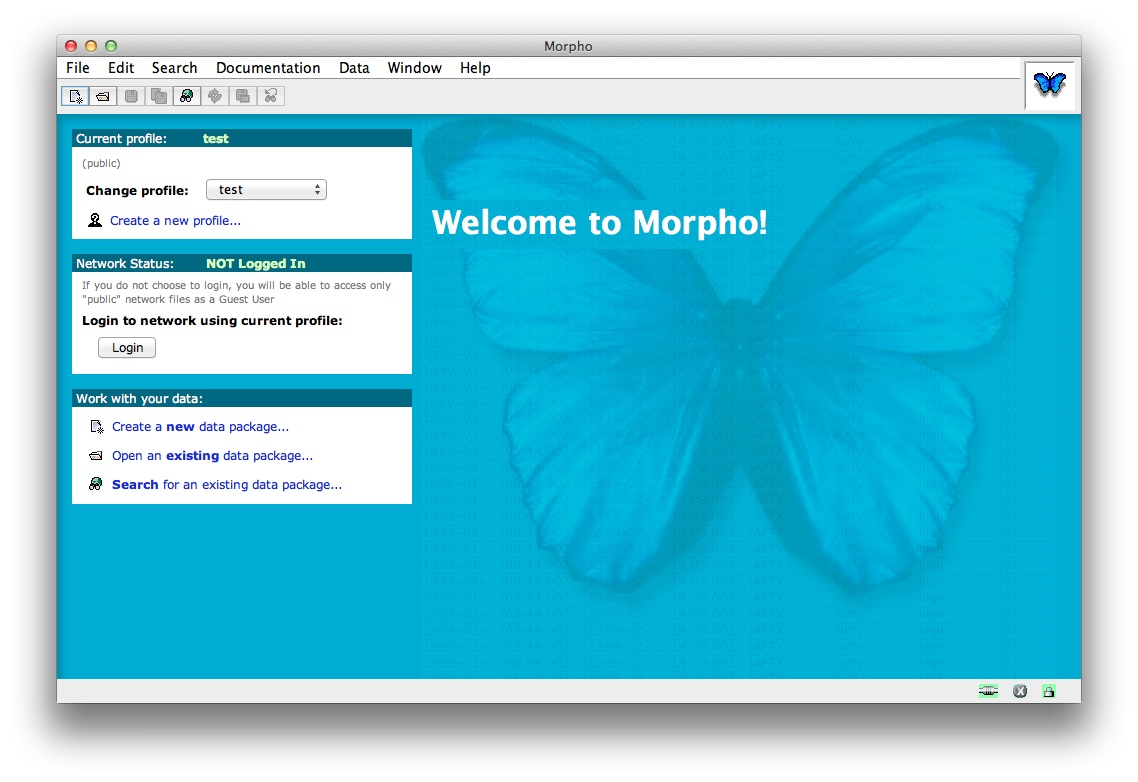
\includegraphics[width=0.7\textwidth]{images/main.jpg}
  \caption{Main Morpho screen with interface components highlighted.}
  \label{fig:main}
\end{figure}

\subsection{Panels}

The Main Morpho screen contains three panels designed to help you easily
log in to a network, select or change a profile, and access the most
common Morpho functions.

\subsubsection[Current profile]{Current Profile Panel}
\label{sec:panel-profile}

The Current Profile panel (\autoref{fig:panel-profile}) contains
information about your current user profile as well as the KNB login
information associated with that profile. Your KNB username is the name
appearing after the ``uid='' just below the title bar of the ``Current
Profile'' panel. 

\begin{figure}
  \centering
    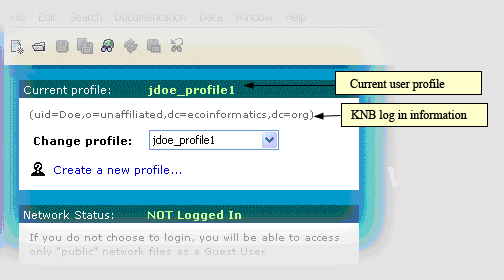
\includegraphics[width=0.7\textwidth]{images/panel-profile.jpg}
  \caption{The Current Profile panel from the Main Morpho screen.}
  \label{fig:panel-profile}
\end{figure}

Use the drop-down menu beside ``Change profile\ldots'' to select a
different profile, or click the ``Create a new profile\ldots'' link to
create a new profile. You may wish to create new profiles to allow
different users to use the same copy of Morpho or to manage different
projects, for example.
%TODO: say something *here* about removing profiles? (we briefly say
%something in the 'getting started' section already, although it seems
%less relevant there because the section is otherwise only about the
%stuff you do when you start Morpho for the first time

\subsubsection[Network Status]{Network Status Panel}
\label{sec:panel-network-status}

The Network Status panel displays the current network status and allows
you to log in and out of the KNB network. The panel offers different
options depending on whether or not you are logged in to the network
(\autoref{fig:panel-network-status}).

\begin{figure}
  \centering
    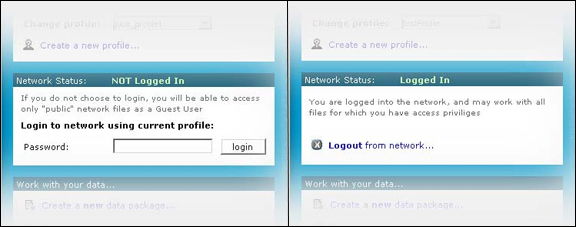
\includegraphics[width=0.7\textwidth]{images/panel-network-status.jpg}
  \caption{The Network Status panel from the Main Morpho screen. The
    image on the left displays the panel as it appears when not logged
    in to the KNB network. The image on the right displays the panel as
    it appears when logged in to the network.}
  \label{fig:panel-network-status}
\end{figure}

If you are not logged in to the KNB network, you can log in by typing
your KNB password in the ``Password'' field and clicking the ``Login''
button. You will be logged in with the KNB username associated with the
current profile (the KNB account information is displayed in the
``Current Profile'' panel). Note that the KNB username is not necessarily
the same as your user profile name. Log out at any time by clicking 
``Logout from network.''

\subsubsection[Work with your data\ldots]{Work with Your Data Panel}
\label{sec:panel-work}

The ``Work with your data\ldots'' panel (\autoref{fig:panel-work})
allows you to easily access the most common features of Morpho. Click
any of the links \hyperref[sec:creating]{Create a new data package},
\hyperref[sec:viewing]{Open an existing data package}, or
\hyperref[sec:searching]{Search for an existing data package} (both
locally and on the KNB network) to start working. Detailed descriptions
of these functions are provided later in the guide.

\begin{figure}
  \centering
    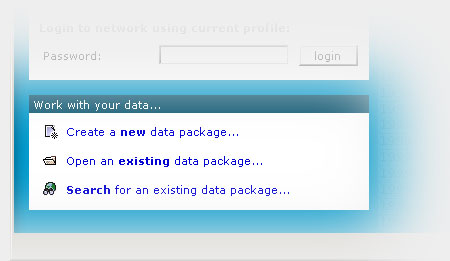
\includegraphics[width=0.7\textwidth]{images/panel-work.jpg}
  \caption{The Work with your data panel from the Main Morpho screen.}
  \label{fig:panel-work}
\end{figure}


\subsection{Menu bar} \label{sec:menu-bar}

The menus in the Menu bar allow you to access all the available Morpho
operations. Each of the menus -- File, Edit, Search, Documentation,
Data, Window, and Help -- is discussed in more detail below.

\subsubsection{File menu} \label{sec:menu-file}

Use the File menu (\autoref{fig:menu-file}) to create a new data
package, open an existing data package, log in and out of the KNB
network, create a new user profile, save a data package, delete a data
package, print documentation, set preferences, and exit Morpho, among
other options. 

\begin{figure}
  \centering
    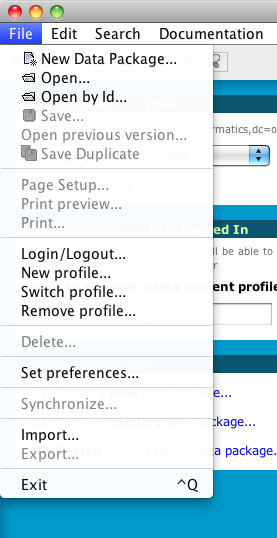
\includegraphics[width=0.5\textwidth]{images/menu-file.png}
  \caption{The File menu}
  \label{fig:menu-file}
\end{figure}

\subsubsection{Edit menu} \label{sec:menu-edit}

Use the Edit menu (\autoref{fig:menu-edit}) to cut, copy or paste items,
as well as reverse changes you have made to a data table or to a set of
data tables.

\begin{figure}
  \centering
    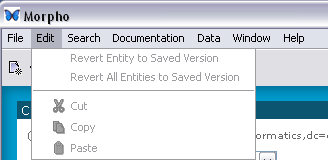
\includegraphics[width=0.5\textwidth]{images/menu-edit.jpg}
  \caption{The Edit menu}
  \label{fig:menu-edit}
\end{figure}

\subsubsection{Search menu} \label{sec:menu-search}

Use the Search menu (\autoref{fig:menu-search}) to search for data
packages, save a search for future use, refine a search by changing
search parameters, or refresh the current search. 

\begin{figure}
  \centering
    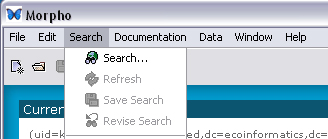
\includegraphics[width=0.5\textwidth]{images/menu-search.jpg}
  \caption{The Search menu.}
  \label{fig:menu-search}
\end{figure}

\subsubsection{Documentation menu} \label{sec:menu-documentation}

Use the Documentation menu (\autoref{fig:menu-documentation}) to add,
delete, or change a variety of different types of documentation
(metadata) for your data package. 

\begin{figure}
  \centering
    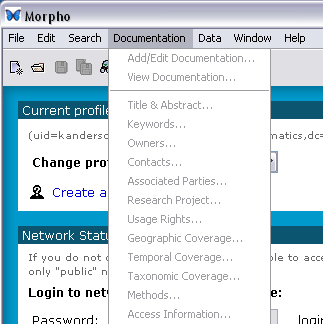
\includegraphics[width=0.5\textwidth]{images/menu-documentation.jpg}
  \caption{The Documentation menu}
  \label{fig:menu-documentation}
\end{figure}

\subsubsection{Data menu} \label{sec:menu-data}

Use the Data menu (\autoref{fig:menu-data}) to import data (e.g., a data
table or an image) or create a data table. You can also edit and
manipulate the data in a data table or add or edit the table
documentation. 

\begin{figure}
  \centering
    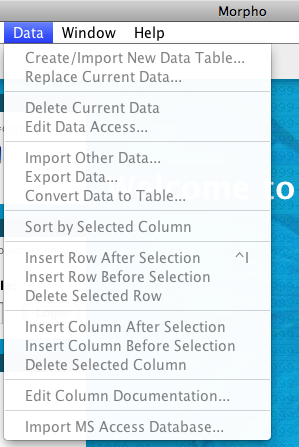
\includegraphics[width=0.5\textwidth]{images/menu-data.png}
  \caption{The Data menu}
  \label{fig:menu-data}
\end{figure}

\subsubsection{Window menu} \label{sec:menu-window}

Use the Window menu (\autoref{fig:menu-window}) to view open Morpho
windows. 

\begin{figure}
  \centering
    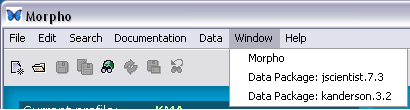
\includegraphics[width=0.5\textwidth]{images/menu-window.jpg}
  \caption{The Window menu.}
  \label{fig:menu-window}
\end{figure}

\subsubsection{Help menu} \label{sec:menu-help}

Use the Help menu (\autoref{fig:menu-help}) to access the Morpho User
Guide (which is what you are now reading). The ``About...'' item
contains general information about Morpho. The ``Intro to Metadata...''
document explains what metadata is and why it is important, as well as
some of the challenges associated with creating it, what Ecological
Metadata Language (EML) is, and how it is used. The EML Specification
contains information about each EML module and how it is used.

\begin{figure}
  \centering
    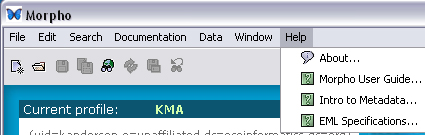
\includegraphics[width=0.5\textwidth]{images/menu-help.jpg}
  \caption{The Help menu}
  \label{fig:menu-help}
\end{figure}
 

\subsection{Toolbar} \label{sec:toolbar}

The Toolbar (\autoref{fig:button-bar-main}) contains shortcut buttons to the
most commonly-used Menu items. Each button is described in
\autoref{tab:button-bar}. To display the purpose of a Morpho button,
simply place your mouse cursor over the button. A small pop-up reminder
will display the purpose of the button.

\begin{figure}
  \centering
    
\includegraphics[width=0.7\textwidth]{images/button-bar-main.png}
  \caption{The Morpho Toolbar}
  \label{fig:button-bar-main}
\end{figure}
 
\begin{table}[ht]
  \centering
  \begin{tabular}{|c|m{0.7\textwidth}|}
  \hline
  \textbf{Button} & \textbf{Description} \\
  \hline
  
\includegraphics[scale=0.7]{images/button-new-dp.png} &
  The ``Create a new data package'' button starts a wizard that guides
  you through the process of creating a new data package. \\
  \hline
  
\includegraphics[scale=0.7]{images/button-open.png} &
  The ``Open\ldots'' button opens an existing data package (provided you
  have adequate access permissions). \\
  \hline
  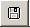
\includegraphics[scale=0.7]{images/button-save.png} &
  The ``Save\ldots'' button saves the current data package either
  locally or on the network. \\
  \hline
  
\includegraphics[scale=0.7]{images/button-duplicate.png} &
  The ``Duplicate this data package and save locally'' button copies the
  current data package. The duplicate can be used as a template to
  create similar data packages. \\
  \hline
  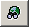
\includegraphics[scale=0.7]{images/button-search.png} &
  The ``Search for data'' button begins the data package search process.
  If logged in to the KNB, you can search both locally and on the KNB
  network. \\
  \hline
  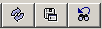
\includegraphics[scale=0.7]{images/button-bar-search.png} &
  The ``Refresh…'', ``Save search,'' and ``Revise search'' buttons are
  enabled only when the screen contains search results. \\
  \hline
  \end{tabular}
  \caption{The Toolbar buttons}
  \label{tab:button-bar}
\end{table}


\subsection{Status Bar} \label{sec:status-bar}

The status bar at the bottom of the Morpho window
(\autoref{fig:status-bar}) contains information about the current status
of various Morpho settings and parameters.

\begin{figure}
  \centering
    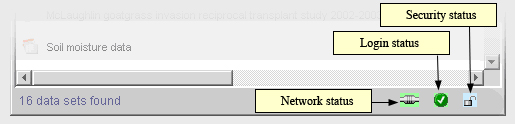
\includegraphics[width=0.7\textwidth]{images/status-bar.jpg}
  \caption{The Morpho Status bar.}
  \label{fig:status-bar}
\end{figure}

\subsubsection*{Network Status}
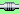
\includegraphics[scale=0.9]{images/indicator-online.png} \hspace{1em}
  Network connection available\\

\includegraphics[scale=0.9]{images/indicator-offline.png} \hspace{1em}
  Network connection not available

\subsubsection*{Login Status}

\includegraphics[scale=0.9]{images/indicator-logged-in.png} \hspace{1em}
  Logged in to network\\

\includegraphics[scale=0.9]{images/indicator-not-logged-in.png} \hspace{1em}
  Not logged in to network

\subsubsection*{Security}

\includegraphics[scale=0.9]{images/indicator-ssl.png} \hspace{1em}
  Using secure (SSL) connection\\

\includegraphics[scale=0.9]{images/indicator-nossl.png} \hspace{1em}
  Not using secure (SSL) connection

